
\documentclass[12pt, a4paper]{article}
\usepackage[top=3cm, bottom=4.25cm, left=2.25cm, right=2.25cm]{geometry}
\usepackage[english]{babel}
\usepackage{blindtext}
\usepackage{hyperref}
\usepackage{graphicx}
\graphicspath{ {./images/} }
\begin{document}

    \title{$\textrm{\LaTeX \  Exercises}$}
    
    \date{}
    \maketitle
    \section{Basic $\textrm{\LaTeX} \textrm { Stuff}$}
    \begin{enumerate}
    \item Create a new directory called \texttt{LatexIntroPaper}.
    \item Create a new .tex file called \texttt{latex-example.tex} in your \texttt{LatexIntroPaper} directory.
    \item Open the file with emacs and make a very simple document with some text. Specify the \texttt{documentclass} to be “article.”
    \item Add title, author, and date information and make a title appear at the top of the page.
    \item Include some \textbf{bold} and \textit{italic} text. Experiment with other font styles like \texttt{this}.
    \item Include a manual line break like this \\ and \\
    \begin{center}
       center some text.
    \end{center}
    \item Add a bulleted and numbered list somewhere in your document. See if you can figure out how to nest them. 
    \begin{itemize}
        \item See, isn’t this better than Word? 
        \item Everything is just so much prettier... 
    \end{itemize}
    \item Generate a .pdf file using \texttt{pdflatex} and view it using \texttt{acroread}.
    \end{enumerate}
    \section{Sections and Referencing}
    \begin{enumerate}
        \item Add to your document three sections, a few subsections, and a subsubsection.
        \item  Label one of the sections you created and create a reference to this section. You should have something like this: In Section 1 you should have made a simple document. Add another label and reference to see that $\textrm{\LaTeX }$ takes care of the numbering for you.
        \item  Create some footnotes.\footnote{Listen to your tutors!}
        \item Add a few citations and create a bibliography section at the bottom of your paper\cite{reference}. Note you may need to compile your .tex file twice to get the citations to appear properly.
  
    \end{enumerate}
     
    \section{Figures and Tables}
    \begin{enumerate}
        \item Create a table to your document. Then add a caption and reference. Try creating something like Table 1.
       
            \begin{table}[h]
                \begin{center}
                    \begin{tabular}{ |r |l| l| }
                        \hline
                     11:00 & Bedckeck & Don’t miss it or your counselor will embarass you!  \\ \hline
                     11:30–? & Fun & The fun starts after bedcheck! \\ \hline
                     ??? & Sleep & It’s hard to find time. \\ \hline
            
                    \end{tabular}
          
                    \caption{This is a pretty table.}
          
                 \end{center}
           
         
             \end{table}
    
       
        \item  Add an figure of any kind to your document. Again add a caption and reference. Note that not all image formats are supported by \texttt{pdflatex}. Recommended file formats are .png and .jpg. Do NOT use .eps or .gif files, as these don’t work with \texttt{pdflatex}. It’s easy to convert from one file format to another; use the command convert file.ext1 \texttt{file.ext2}. For example, to convert \texttt{image.gif} to \texttt{image.png} just type \texttt{convert image.gif image.png}.
        
       \begin{figure}[h]
            \centering
            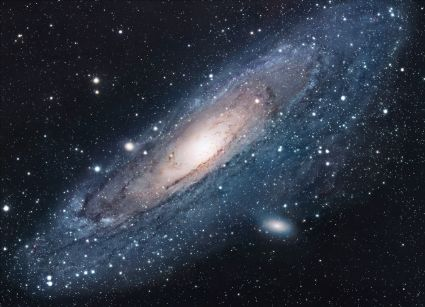
\includegraphics[scale=3]{universe}
            \caption {Your dorm!}
        \end{figure}
    
    \end{enumerate}
    \newpage
    \section{Math Mode}
    \begin{enumerate}
        \item  The real power of $\textrm{\LaTeX }$ is with its ability to format math expressions. Write whatever cool math equation you’d like.
        \item Write some inline math expressions as well: $E=mc^2$
        \item Experiment with other symbols and operators. You can find a lot of information about what is possible with math mode here:\\ \\
    \href{http://www.ams.org/publications/authors/tex/amslatex}{\texttt{http://www.ams.org/tex/amslatex.html}}\\ \\ 
    .
    \end{enumerate}
    \section{Looking Stuff Up}
    It’s impossible to cover everything that $\textrm{\LaTeX }$ can do in a few days. But luckily its very easy to figure out how to do something we haven’t covered (or you forgot about). Just Google it! You’ll be happily suprised how easy it is to find examples for exactly what you’re looking for. If you are still stuck, \textit{someone} will be able to help you. Also check out the following: 
    \begin{itemize}
        \item Art of Problem Solving:\\ \\
        \href{https://artofproblemsolving.com/LaTeX/AoPS_L_About.php}{\texttt{https://artofproblemsolving.com/LaTeX/AoPS\_L\_About.php}}\\ 
        \item  RSI $\textrm{\LaTeX }$ materials on the website:\\ \\
        \href{http://web.mit.edu/rsi/www/}{\texttt{http://web.mit.edu/rsi/www/}}
    \end{itemize}
        
    \begin{thebibliography}{9}
    \bibitem{reference}
     The Gods of RSI.
    
    \end{thebibliography}
\end{document}